\chapter{النبات المدجَّن}\label{ch:g12:domesticated-plants}

إلى جانب كوز ذرة حديث --- ستمئة حبة في صفوف مرتبة، ملفوفة في أغلفة،
ممسوكة على قالب لا يطلقها --- وضع سنبل التيوسنت، وهي الحشيشة البرية
التي جاء منها: اثنتا عشرة حبة في صف واحد، كل واحدة في غلاف حجري، تسقط
واحدة واحدة عند النضج. تسعة آلاف سنة من الاختيار، بمزارعين حفظوا بذور
النباتات التي فضلوها، حوّلت هذا إلى ذاك. والحاصل لا يستطيع أن ينجو
موسمًا واحدًا من دوننا: فكوز ذرة يترك في حقل يعفن حيث هو. وهذا الفصل في
ما يحل بنبات حين يصير الناس بيئته المنتقية --- وفي الطرق الأحدث إلى
تغيير \omterm{def:g10:universal-dna:gene}{مورّثات} نبات عمدًا.

\section{انتقاء يقوم به الناس}

\begin{definition}[التدجين والانتقاء الاصطناعي]\label{def:g12:domesticated-plants:domestication}
\emph{التدجين}\index{تدجين} تحويل \omterm{def:g10:biodiversity-scales:species}{نوع} بري إلى \omterm{def:g10:biodiversity-scales:species}{نوع} يعتمد على البشر
ويخدمهم، \emph{بالانتقاء الاصطناعي}\index{انتقاء اصطناعي}: إذ يحفظ
الناس، في كل جيل، بذور الأفراد ذوي الصفات التي يريدونها ويزرعونها،
فترتفع تواترات \omterm{def:g10:universal-dna:gene}{الأليلات} وراء تلك الصفات. وهو انتقاء
\cref{ch:g12:selection-drift-speciation} بعين بشرية بدل البيئة، ويعمل
بالحساب نفسه --- أسرع، إذ يكون الانتقاء مقصودًا وشديدًا.
\end{definition}

\begin{proposition}[ما الذي ينتقيه التدجين]\label{prop:g12:domesticated-plants:traits}
تشترك المحاصيل في طقم من الصفات ما كان نبات بري ليبقيها، هو
\emph{متلازمة \omterm{def:g12:domesticated-plants:domestication}{التدجين}}: بذور تبقى على النبات بدل أن تتناثر (سنبلة لا
تتفتت)؛ وبذور وثمار أكبر؛ وبذور تنبت في الحال بدل أن تنتظر سنين في
التربة؛ وفقد السموم والدفاعات المرة؛ ونبات مكتنز قليل الأفرع له سنبلة
واحدة كبيرة بدل سنابل صغيرة كثيرة؛ ونضج متزامن. وكل واحدة منها نافعة
للحاصد ضارة بنبات قائم بنفسه --- فالمحصول نبات منتقًى لراحتنا وضد
استقلاله.
\end{proposition}
\begin{proof}[شواهد]
القمح البري ينثر حبوبه من ساق هش؛ وأول القموح المزروعة، الموجودة في
أقدم مواقع الزراعة، لها ساق متين يمسك الحب --- فمنجل الحاصد انتقى، بلا
قصد، الطافرات التي بقي حبها على النبات ليجمع ويزرع. والتيوسنت والذرة
لا يختلفان إلا في نحو خمس \omterm{def:g10:universal-dna:gene}{مورّثات} كبرى: واحدة تحوّل نباتًا كثير الأفرع
إلى ساق واحد، وأخرى تحرر الحبة من غلافها الحجري، وأخريات تكثر الصفوف.
وتهجين الاثنين يعطي نسلًا خصيبًا، والصور الوسيطة موجودة: أي \omterm{def:g10:biodiversity-scales:species}{النوع}
نفسه، معادًا تشكيله.
\end{proof}

\begin{omfigure}
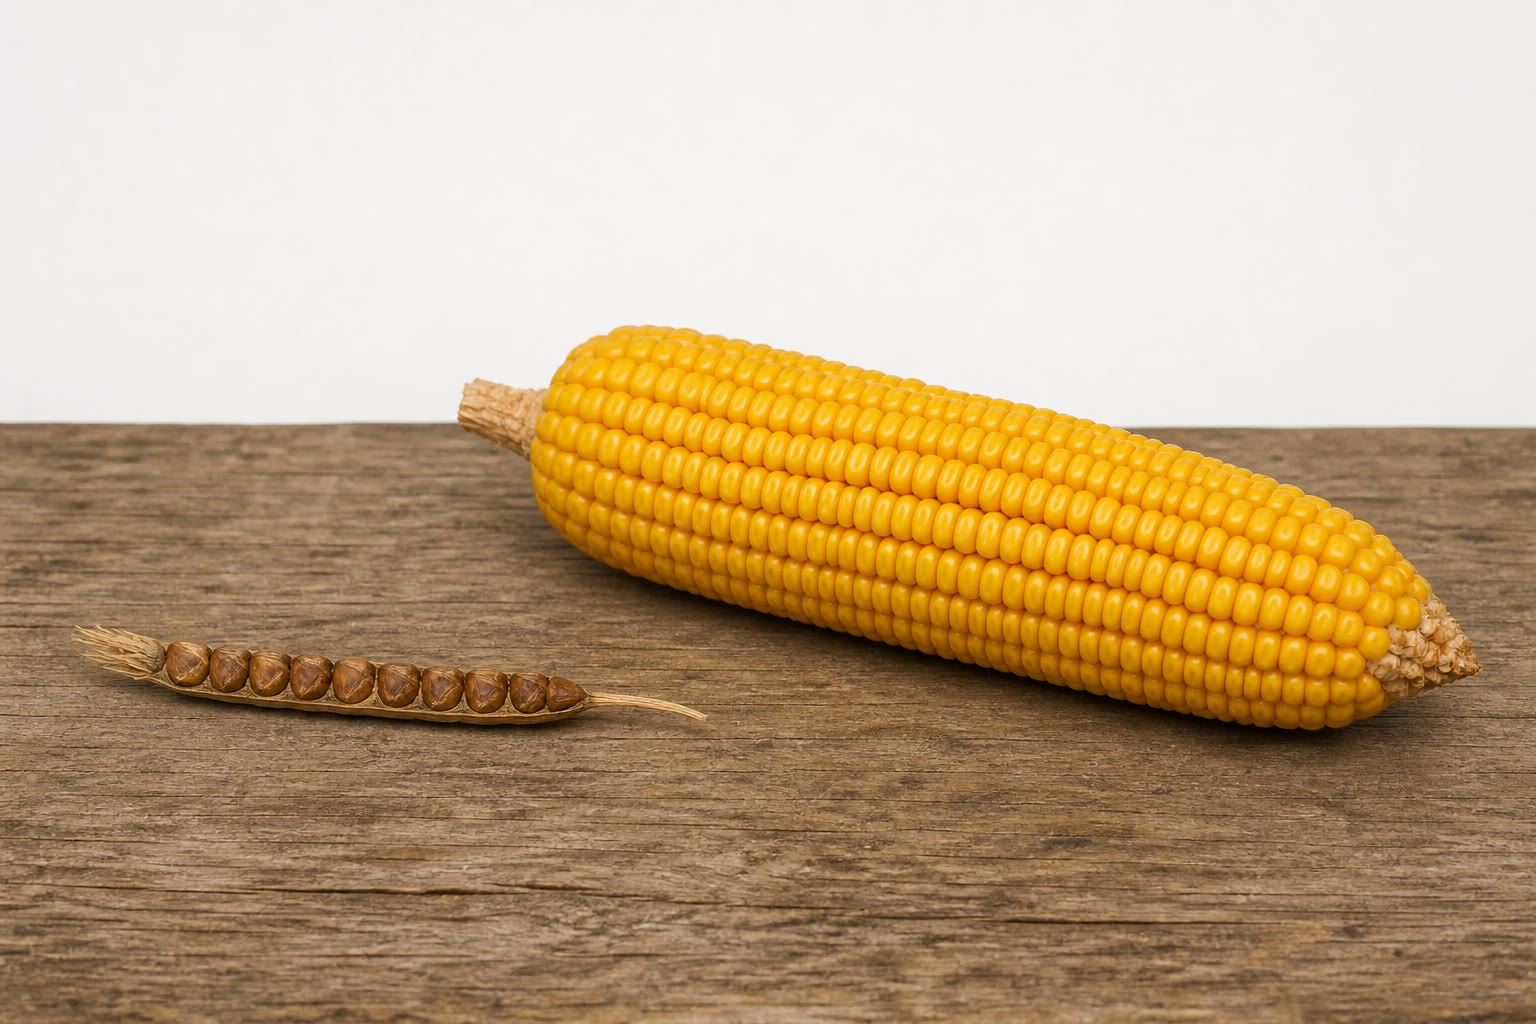
\includegraphics[width=0.62\linewidth]{images/book2/ai/g12-domestic-teosinte-maize.jpg}

{\small التيوسنت والذرة. اثنتا عشرة حبة مغلَّفة في صف واحد على سنبلة
هشة، في مقابل مئات الحبات العارية ممسوكة على قالب: تسعة آلاف سنة من
الاختيار، وحفنة من \omterm{def:g10:universal-dna:gene}{المورّثات}.}
\end{omfigure}

\begin{omfigure}
\begin{tikzpicture}[font=\small, >=Stealth,
  b/.style={draw, rounded corners, align=center, text width=2.2cm, minimum height=0.9cm}]
  \node[b, fill=omMeth!15, text width=2.8cm] (wild) at (0,0) {الكرنب البري\\ (نوع واحد)};
  \node[b, fill=omDef!12] (kale) at (5,3.0) {الكرنب الأجعد:\\ الأوراق};
  \node[b, fill=omDef!12] (cab) at (5,1.8) {الملفوف:\\ البرعم القمي};
  \node[b, fill=omDef!12, text width=2.7cm] (spr) at (5,0.6) {كرنب بروكسل:\\ البراعم الجانبية};
  \node[b, fill=omDef!12] (kohl) at (5,-0.6) {الكرنب اللفتي:\\ الساق};
  \node[b, fill=omDef!12] (broc) at (5,-1.8) {البروكلي:\\ براعم الأزهار};
  \node[b, fill=omDef!12] (cauli) at (5,-3.0) {القرنبيط:\\ حوامل الأزهار};
  \foreach \t in {kale,cab,spr,kohl,broc,cauli} \draw[->] (wild.east) -- (\t.west);
  \node[anchor=west, align=left, text width=4.6cm] at (7.2,0) {ستة محاصيل، ونوع واحد: ففي كل سلالة انتقى المزارعون تضخيم عضو مختلف. والستة كلها ما زالت تتناسل فيما بينها.};
\end{tikzpicture}

{\small \omterm{def:g12:domesticated-plants:domestication}{الانتقاء الاصطناعي} من \omterm{def:g10:biodiversity-scales:species}{نوع} بري واحد. فانتقاء الأوراق أو البراعم
أو الساق أو الأزهار في سلالات مختلفة أنتج نباتات تبدو أنواعًا مختلفة
وليست كذلك.}
\end{omfigure}

\begin{example}[ما الذي فقده المحصول]\label{ex:g12:domesticated-plants:lost}
الذرة لا تستطيع أن تنثر بذرها؛ والقمح المزروع لا يستطيع أن ينفض حبه؛
والموز والعنب عديم البذر لا يصنعان بذورًا البتة ويكثران بالعقل، فكل
نبتة نسيلة. فبقاء المحصول موكول إلى المزارع، و\emph{تنوعه الوراثي}
انكمش مع كل مرحلة من الانتقاء: فالصنف الحديث يكاد يكون متجانسًا، وقد
تزرع منطقة كاملة صنفًا واحدًا. والأقرباء البريون، وهم ما زالوا متنوعين،
هم حيث تحفظ \omterm{def:g10:universal-dna:gene}{الأليلات} التي قد يحتاجها محصول المستقبل --- لمرض جديد،
أو لمناخ أجف --- (\cref{ch:g10:biodiversity-scales}).
\end{example}

\section{التربية بالتهجين}

\begin{proposition}[الأصناف والهجن]\label{prop:g12:domesticated-plants:hybrids}
يصنع المربّون أصنافًا جديدة بتهجين نباتات تحمل \omterm{def:g10:universal-dna:gene}{أليلات} نافعة مختلفة، ثم
انتقاء التوافيق التي يريدونها بين النسل، عبر أجيال عدة. وحالة خاصة
تسود الذرة وكثيرًا من الخضر: هي \emph{الهجين F1}\index{هجين F1}. إذ
تهجَّن سلالتان نقيتان --- جعلت كل منهما متجانسة متماثلة \omterm{def:g10:universal-dna:gene}{الأليلات}
بأجيال من التلقيح الذاتي --- فيأتي نسلهما متطابقًا وراثيًا كله، متغاير
\omterm{def:g10:universal-dna:gene}{الأليلين} عند كل \omterm{def:g10:universal-dna:gene}{مورّثة} تختلف فيها السلالتان، وأقوى وأغزر إنتاجًا من
أي من الوالدين بوضوح. فإذا زرع ثانية، انعزل بذر الهجين نفسه إلى خليط
من نباتات أقل قوة: فيشتري المزارع بذرًا هجينًا جديدًا كل سنة.
\end{proposition}
\admitted

\begin{omfigure}
\begin{tikzpicture}[font=\small, >=Stealth,
  b/.style={draw, rounded corners, align=center, text width=2.6cm, minimum height=1.0cm}]
  \node[b, fill=omDef!12] (a) at (0,1.2) {السلالة النقية A\\ $AA\,bb$، متجانسة};
  \node[b, fill=omDef!12] (bb) at (0,-1.2) {السلالة النقية B\\ $aa\,BB$، متجانسة};
  \node[b, fill=omMeth!20, text width=3.0cm] (f1) at (4.6,0) {الهجين F1\\ $Aa\,Bb$، متطابق كله،\\ وقوي};
  \node[b, fill=omProp!15, text width=3.4cm] (f2) at (9.6,0) {F2 من بذر الهجين:\\ $AA$ و$Aa$ و$aa$ \dots مختلط،\\ ومردود أدنى 15--20\%};
  \draw[->] (a) -- (f1); \draw[->] (bb) -- (f1);
  \draw[->] (f1) -- node[above] {يزرع من بذره} (f2);
\end{tikzpicture}

{\small \omterm{prop:g12:domesticated-plants:hybrids}{الهجين F1}. سلالتان متماثلتا \omterm{def:g10:universal-dna:gene}{الأليلات} تعطيان نسلًا متجانسًا
متغاير \omterm{def:g10:universal-dna:gene}{الأليلين} عالي القوة؛ والجيل التالي ينعزل ويفقدها، فوجب شراء
البذر من جديد كل سنة --- وهو أساس صناعة البذور.}
\end{omfigure}

\begin{omfigure}
\begin{tikzpicture}
\begin{axis}[
  width=0.86\linewidth, height=5.6cm,
  axis x line=bottom, axis y line=left,
  xmin=1900, xmax=2025, ymin=0, ymax=9,
  xlabel={السنة}, ylabel={مردود القمح (t/ha)},
  xlabel style={font=\small, at={(axis description cs:0.5,-0.12)}, anchor=north},
  ylabel style={font=\small},
  tick label style={font=\small}, xtick={1900,1925,1950,1975,2000,2025}, ytick={0,2,4,6,8},
  clip=false,
]
\addplot[thick, omMeth, mark=*, mark size=1.5pt] coordinates
  {(1900,1.3) (1920,1.4) (1940,1.6) (1950,1.9) (1960,2.6) (1970,3.6) (1980,5.0) (1990,6.5) (2000,7.2) (2010,7.3) (2020,7.5)};
\draw[dashed, gray] (axis cs:1955,0) -- (axis cs:1955,8.5);
\node[font=\scriptsize, anchor=south, align=center] at (axis cs:1955,8.5) {أصناف قصيرة القش،\\ وأسمدة، ومبيدات};
\end{axis}
\end{tikzpicture}

{\small متوسط مردود القمح في بلد من غرب أوروبا على مدى قرن (مدوَّرًا).
ثابت خمسين سنة، ثم تضاعف أربع مرات في أربعين سنة بأصناف ربّيت لتحمل
سنابل ثقيلة على سوق قصيرة، مع الأسمدة ومكافحة الآفات. أما الاستواء منذ
سنة 2000 فهو موضوع التربية الجارية.}
\end{omfigure}

\begin{example}[لماذا كان الهجين قويًا، ولماذا لا يدوم]\label{ex:g12:domesticated-plants:vigour}
كل سلالة نقية، وهي متماثلة \omterm{def:g10:universal-dna:gene}{الأليلات} في كل مكان، تحمل بعض \omterm{def:g10:universal-dna:gene}{الأليلات}
المتنحية الضعيفة بجرعة مضاعفة؛ وتهجين سلالتين يحجب \omterm{def:g10:universal-dna:gene}{أليلات} كل سلالة
الضعيفة وراء \omterm{def:g10:universal-dna:gene}{أليلات} الأخرى العاملة، عند كل \omterm{def:g10:universal-dna:gene}{مورّثة} تختلفان فيها.
فالجيل F1 متغاير \omterm{def:g10:universal-dna:gene}{الأليلين} ومن ثم قوي. وفي الجيل التالي، يوزع \omterm{def:g12:meiosis-genetic-shuffling:meiosis}{الانقسام
المنصّف} والإخصاب \omterm{def:g10:universal-dna:gene}{الأليلات} من جديد
(\cref{ch:g12:meiosis-genetic-shuffling}): فيصير ربع النباتات متماثل
\omterm{def:g10:universal-dna:gene}{الأليلات} \omterm{def:g10:universal-dna:gene}{للأليل} الضعيف عند كل \omterm{def:g10:universal-dna:gene}{مورّثة}، ويصير الحقل رقعًا.
\end{example}

\section{تغيير المورّثات مباشرة}

\begin{proposition}[المحاصيل المنقولة المورّثات والمحرَّرة]\label{prop:g12:domesticated-plants:transgenic}
منذ ثمانينيات القرن العشرين صار في الوسع إدخال \omterm{def:g10:universal-dna:gene}{مورّثة} في نبات من غير
تهجين: وهو \emph{النقل المورّثي}\index{نقل مورّثي}
(\cref{ch:g10:universal-dna}). وتستعمل مركبةً جرثومةُ تربة تحقن
بطبيعتها قطعة من \omterm{def:g10:universal-dna:information}{DNA} خاصتها في \omterm{def:g10:cells-common-unit:cell}{خلايا} النبات: فتدرج \omterm{def:g10:universal-dna:gene}{المورّثة} المطلوبة
في تلك القطعة، وتعدى \omterm{def:g10:cells-common-unit:cell}{خلايا} نباتية، ثم تنمّى نباتات كاملة من \omterm{def:g10:cells-common-unit:cell}{الخلايا}
التي أخذت \omterm{def:g10:universal-dna:gene}{المورّثة}. وقد تأتي \omterm{def:g10:universal-dna:gene}{المورّثة} من أي \omterm{def:g10:biodiversity-scales:species}{نوع}. وحديثًا، صار في الوسع
تعديل \omterm{def:g10:universal-dna:gene}{مورّثات} النبات نفسه عند موضع مختار --- وهو \emph{تحرير
\omterm{def:g10:universal-dna:gene}{المورّثات}} --- من غير إضافة \omterm{def:g10:universal-dna:information}{DNA} غريب. والصفات حتى الآن: مقاومة حشرة
(\omterm{def:g10:universal-dna:gene}{مورّثة} سم جرثومي)، وتحمّل مبيد أعشاب، ومقاومة فيروس، وطليعة فيتامين
في الأرز، وزيوت مغيَّرة التركيب.
\end{proposition}
\admitted

\begin{omfigure}
\begin{tikzpicture}[font=\small, >=Stealth,
  b/.style={draw, rounded corners, align=center, text width=2.4cm, minimum height=1.0cm}]
  \node[b, fill=omThm!12] (gene) at (0,0) {المورّثة المطلوبة\\ (من أي نوع)};
  \node[b, fill=omProp!15] (bact) at (3.3,0) {تدرج في DNA\\ تنقله إلى النبات\\ جرثومة تربة};
  \node[b, fill=omDef!12] (cells) at (6.6,0) {تعدى خلايا نباتية؛\\ وبعضها يأخذ\\ المورّثة};
  \node[b, fill=omMeth!15] (plant) at (9.9,0) {تنمّى نباتات كاملة\\ من تلك الخلايا:\\ منقولة المورّثات};
  \draw[->] (gene) -- (bact); \draw[->] (bact) -- (cells); \draw[->] (cells) -- (plant);
\end{tikzpicture}

{\small صنع نبات منقول \omterm{def:g10:universal-dna:gene}{المورّثات}. جرثومة تدرج بطبيعتها \omterm{def:g10:universal-dna:information}{DNA} في \omterm{def:g10:cells-common-unit:cell}{خلايا}
النبات تحمل \omterm{def:g10:universal-dna:gene}{المورّثة} المختارة إلى الداخل؛ ثم تجدَّد نباتات من \omterm{def:g10:cells-common-unit:cell}{الخلايا}
التي تلقتها، وتنقلها هذه عبر بذورها.}
\end{omfigure}

\begin{example}[مورّثة سم في الذرة]\label{ex:g12:domesticated-plants:bt}
جرثومة تربة تصنع بروتينًا سامًا لليرقات غير ضار بالثدييات؛ ومورّثتها،
إذا أدرجت في الذرة، جعلت كل \omterm{def:g10:cells-common-unit:cell}{خلية} من \omterm{def:g10:cells-common-unit:cell}{خلايا} النبات تنتج السم، فتموت
يرقات الثاقبة التي تنفق السوق عند أول قضمة. فيقل رش المبيدات؛ وترتفع
المردودات حيث كانت الثاقبة شديدة. وفي غضون عقد، ظهرت ثاقبات مقاومة
للسم حيث زرع المحصول بلا انقطاع --- أي انتقاء
\cref{ch:g11:antibiotic-resistance} في حقل --- وصار المزارعون ملزمين
بزرع ملاجئ من الذرة العادية إلى جانب المنقولة \omterm{def:g10:universal-dna:gene}{المورّثات}، حتى تنجو
ثاقبات حساسة تخفّف المقاومة.
\end{example}

\section{اختيارات}

\begin{proposition}[ما هو على المحك]\label{prop:g12:domesticated-plants:stakes}
كل تقنية من تقنيات هذا الفصل تثير الأسئلة نفسها في صورة جديدة: تضيّق
التنوع (صنف واحد في منطقة، \omterm{def:g10:universal-dna:gene}{ومورّثة} واحدة في كل نبتة)، واعتماد المزارعين
على بذر لا يستطيعون حفظه، وانتقاء الآفات والأعشاب المقاومة لدفاعات
المحصول، وانتقال \omterm{def:g10:universal-dna:gene}{مورّثات} المحصول إلى أقربائه البريين بغبار الطلع، وسلامة
ما يؤكل وملكيته. ولا يجيب عن أي منها علم الأحياء وحده؛ فالأحياء تقول
ما تفعله كل تقنية وما لا تفعله، وماذا تنتقي.
\end{proposition}
\admitted

\begin{method}[قراءة تاريخ محصول]\label{met:g12:domesticated-plants:read}
\begin{enumerate}
  \item عيّن السلف البري وما فقده المحصول قياسًا به (الانتشار، والسكون،
        والدفاعات، والتنوع).
  \item عيّن كيف أجري التغيير: انتقاء غير واع بالحصاد، أم انتقاء
        مقصود، أم تهجين وانتقاء، أم تهجين بين نوعين، أم \omterm{prop:g10:universal-dna:universal}{نقل مورّثي}، أم
        تحرير.
  \item أحص \omterm{def:g10:universal-dna:gene}{المورّثات} المعنية حيث تعرف: بضع \omterm{def:g10:universal-dna:gene}{مورّثات} كبرى لمتلازمة
        \omterm{def:g12:domesticated-plants:domestication}{التدجين}، وكثير من الصغرى للمردود، وواحدة لصفة منقولة.
  \item اسأل على ماذا صار المحصول يعتمد (المزارع، والبذر المشترى،
        ومبيد الأعشاب، والملاجئ) وما الذي يعتمد عليه.
\end{enumerate}
\end{method}

\begin{remark}[أقدم تجربة في التطور]\label{rem:g12:domesticated-plants:oldest}
افتتح داروين كتابه في أصل \omterm{def:g10:biodiversity-scales:species}{الأنواع} بفصل عن الحمام والكرنب، لأن المربّين
كانوا قد بينوا أصلًا ما يستطيعه الانتقاء في بضعة قرون؛ فلم يبق عليه
إلا أن ينزع المربّي ويطيل الزمن. فكل محصول برهان على الفصول الثلاثة
الأخيرة --- التنوع، والانتقاء، وتغير التواترات الذي يبدل نوعًا ---
مُجرى بسرعة بشرية، وسجل نتائجه في كل حقل وكل سوق.
\end{remark}

\section{تمارين}

\begin{exercise}[$\star$]\label{exo:g12:domesticated-plants:1}
عرّف \omterm{def:g12:domesticated-plants:domestication}{التدجين} \omterm{def:g12:domesticated-plants:domestication}{والانتقاء الاصطناعي}.
\end{exercise}

\begin{exercise}[$\star$]\label{exo:g12:domesticated-plants:2}
اذكر أربع صفات من متلازمة \omterm{def:g12:domesticated-plants:domestication}{التدجين} وقل لماذا كانت كل واحدة عائقًا لنبات
بري.
\end{exercise}

\begin{exercise}[$\star$]\label{exo:g12:domesticated-plants:3}
ما \omterm{prop:g12:domesticated-plants:hybrids}{الهجين F1}، ولماذا يشتري المزارعون بذره كل سنة؟
\end{exercise}

\begin{exercise}[$\star$]\label{exo:g12:domesticated-plants:4}
كيف تدخل \omterm{def:g10:universal-dna:gene}{مورّثة} في نبات من غير تهجين؟
\end{exercise}

\begin{exercise}[$\star$]\label{exo:g12:domesticated-plants:5}
من شكل المردود، بأي معامل ارتفع مردود القمح بين سنة 1950 وسنة 2000؟
\end{exercise}

\begin{exercise}[$\star\star$]\label{exo:g12:domesticated-plants:6}
فسّر كيف انتقى الحصاد بالمنجل، بلا أي قصد إلى التربية، قمحًا ذا ساق
متين.
\end{exercise}

\begin{exercise}[$\star\star$]\label{exo:g12:domesticated-plants:7}
الكرنب الأجعد والملفوف والبروكلي تتناسل فيما بينها بحرية. أهي \omterm{def:g10:biodiversity-scales:species}{نوع}
واحد أم ثلاثة؟ وما الذي جعلها تبدو بهذا الاختلاف؟
\end{exercise}

\begin{exercise}[$\star\star$]\label{exo:g12:domesticated-plants:8}
تهجَّن سلالتان نقيتان. عند \omterm{def:g10:universal-dna:gene}{مورّثة} تكون فيها السلالة A هي $AA$ والسلالة
B هي $aa$، أعط \omterm{def:g11:enzymes-and-phenotype:phenotype}{النمط الوراثي} للجيل F1 والأنماط الوراثية ونسبها في
الجيل F2. ولماذا كان F1 متجانسًا وF2 غير متجانس؟
\end{exercise}

\begin{exercise}[$\star\star$]\label{exo:g12:domesticated-plants:9}
لماذا ظهرت ثاقبات مقاومة في حقول الذرة المنتجة للسم، وكيف يبطئها ملجأ
من الذرة العادية؟
\end{exercise}

\begin{exercise}[$\star\star$]\label{exo:g12:domesticated-plants:10}
التيوسنت والذرة يختلفان في نحو خمس \omterm{def:g10:universal-dna:gene}{مورّثات} كبرى. فسّر كيف تستطيع
\omterm{def:g10:universal-dna:gene}{مورّثات} بهذه القلة أن تغير النبات هذا التغيير كله، مستعينًا بما في
\cref{ch:g12:diversification-of-life}.
\end{exercise}

\begin{exercise}[$\star\star$]\label{exo:g12:domesticated-plants:11}
لماذا تصان أقرباء المحاصيل البرية في بنوك البذور، مع أن مردودها يكاد
يكون معدومًا؟
\end{exercise}

\begin{exercise}[$\star\star\star$]\label{exo:g12:domesticated-plants:12}
يزرع لفت زيتي متحمل لمبيد أعشاب إلى جانب خردل بري يستطيع أن يتهاجن
معه. تنبأ بما قد يحدث على مدى سنين، وسمّ مسارات الفصول السابقة
المعنية.
\end{exercise}

\begin{exercise}[$\star\star\star$]\label{exo:g12:domesticated-plants:13}
منحني المردود مستو منذ سنة 2000. اقترح سببين أحيائيين وسببًا غير
أحيائي، وقل ماذا قد يجرب مربٍّ.
\end{exercise}

\begin{exercise}[$\star\star\star$]\label{exo:g12:domesticated-plants:14}
قارن، في ثلاث نقاط، صنفًا حصل عليه بالتهجين والانتقاء بصنف حصل عليه
\omterm{prop:g12:domesticated-plants:transgenic}{بالنقل المورّثي}: أصل \omterm{def:g10:universal-dna:gene}{الأليل} الجديد، وعدد \omterm{def:g10:universal-dna:gene}{المورّثات} المغيَّرة، والزمن
المستغرق.
\end{exercise}

\begin{exercise}[$\star\star\star$]\label{exo:g12:domesticated-plants:15}
"\omterm{def:g12:domesticated-plants:domestication}{التدجين} نقيض \omterm{def:g12:selection-drift-speciation:selection}{الانتقاء الطبيعي}." ناقش في فقرة بحساب تواترات \omterm{def:g10:universal-dna:gene}{الأليلات}،
وبعامل الانتقاء، وبمصير النبات المنتقى.
\end{exercise}

\section{مسألة: تسعة آلاف سنة، وخمس مورّثات}

\begin{problem}[{مسألة نهاية الأسبوع --- الذرة تصنع من التيوسنت:
السنابل تقارن، والانتقاء يحسب، ومردود هجين يتابع إلى الجيل F2، ومورّثة
سم تدار في وجه المقاومة}]
\label{pb:g12:domesticated-plants:1}
سنبلة تيوسنت تحمل 12 حبة كتلة كل منها \qty{0.08}{g}، مغلَّفة في قشرة
صلبة، على محور هش؛ وكوز ذرة يحمل 600 حبة كتلة كل منها \qty{0.3}{g}،
عارية، على قالب صلب. وقد دجّنت الذرة قبل نحو 9000 سنة؛ والجيل سنة
واحدة.

\medskip
\noindent\textbf{القسم الأول --- السنابل.}
\begin{enumerate}
  \item احسب كتلة الحب في السنبلة الواحدة عند التيوسنت وعند الذرة،
        والمعامل بينهما.
  \item اذكر صفات كوز الذرة التي تنتمي إلى متلازمة \omterm{def:g12:domesticated-plants:domestication}{التدجين}، وقل عند كل
        واحدة لماذا كانت ستكون عائقًا لنبات بري.
  \item الحبة المغلَّفة تضبطها \omterm{def:g10:universal-dna:gene}{مورّثة} واحدة، \omterm{def:g10:universal-dna:gene}{والأليل} العاري \omterm{def:g11:genes-and-disease:genetic}{متنح}. فسّر
        لماذا لم يكن في وسع أوائل المزارعين أن يجدوا نباتات عارية
        الحب إلا أفرادًا نادرين في حقولهم.
  \item افترض أن تواتر \omterm{def:g10:universal-dna:gene}{الأليل} العاري كان 0.01 في \omterm{def:g12:selection-drift-speciation:population}{الجمهرة} البرية. فأي
        كسر من النباتات أبدى حبًا عاريًا؟
  \item تزرع مزارعة بذرًا من نباتات عارية الحب لا غير. فما تواتر \omterm{def:g10:universal-dna:gene}{الأليل}
        العاري في محصولها التالي؟
\end{enumerate}

\medskip
\noindent\textbf{القسم الثاني --- تسعة آلاف جيل.}
\begin{enumerate}[resume]
  \item ارتفع عدد حبات السنبلة من 12 إلى 600 على مدى 9000 جيل. احسب
        متوسط معامل الزيادة في الجيل الواحد. ولماذا كفى تغير بهذا
        الصغر في الجيل؟
  \item عدد صفوف الحب تضبطه \omterm{def:g10:universal-dna:gene}{مورّثات} كثيرة صغيرة الأثر. فسّر لماذا
        تستجيب صفة كهذه للانتقاء تدريجيًا ومدة طويلة، بينما تغيرت صفة
        الحبة المغلَّفة في خطوة واحدة.
  \item ما زالت الذرة تتهاجن مع التيوسنت وتعطي نسلًا خصيبًا. أهما \omterm{def:g10:biodiversity-scales:species}{نوع}
        واحد؟ وما الذي غيره \omterm{def:g12:domesticated-plants:domestication}{التدجين} وما الذي لم يغيره؟
  \item الصنف الحديث متجانس وراثيًا. اذكر الخطر المترتب على ذلك،
        والمورد الذي يجيب عنه.
  \item الذرة لا تستطيع نشر بذورها. فماذا يستلزم ذلك في العلاقة بين
        النبات والمزارع، من حيث الانتقاء؟
\end{enumerate}

\medskip
\noindent\textbf{القسم الثالث --- الهجين.}
مردود السلالة النقية A \qty{5}{t/ha}، والسلالة B \qty{5.5}{t/ha}،
وهجينهما F1 \qty{10}{t/ha}؛ ومردود الجيل F2 المزروع من بذر الهجين
\qty{8.2}{t/ha}. ويكلف البذر الهجين ما يعادل \qty{0.4}{t/ha}
من الذرة.
\begin{enumerate}[resume]
  \item بأي نسبة مئوية يتجاوز F1 الوالد الأفضل؟ وبأي نسبة مئوية يقصّر
        F2 عن F1؟
  \item فسّر قوة F1 وخسارة F2 بالأنماط الوراثية في
        \cref{ex:g12:domesticated-plants:vigour}.
  \item يتردد مزارع بين شراء بذر هجين كل سنة وحفظ بذر من F1. قارن صافي
        المحاصيل، وقل لماذا توجد تجارة شركة البذور.
  \item لماذا لا تباع السلالات النقية للمزارعين ببساطة ليصنعوا الهجين
        بأنفسهم؟
  \item ماذا فعل نظام الهجن \omterm{def:g10:biodiversity-scales:biodiversity}{بالتنوع الوراثي} في الحقول، وباستقلال
        المزارع؟
\end{enumerate}

\medskip
\noindent\textbf{القسم الرابع --- \omterm{def:g10:universal-dna:gene}{مورّثة} السم.}
\omterm{def:g12:selection-drift-speciation:population}{جمهرة} ثاقبة فيها \omterm{def:g10:universal-dna:gene}{أليل} مقاومة تواتره 0.001، وهو \omterm{def:g11:genes-and-disease:genetic}{متنح}؛ ولا ينجو على ذرة
السم إلا أفراد $rr$.
\begin{enumerate}[resume]
  \item أي كسر من الثاقبات ينجو في حقل ذرة سم في السنة الأولى؟ احسب
        تواتر $r$ بين الناجين.
  \item فسّر لماذا تنتشر المقاومة، بلا ملاجئ، في غضون سنين قليلة،
        مستعينًا بحالة \omterm{def:g11:antibiotic-resistance:antibiotic}{المضادات الحيوية} نموذجًا.
  \item ملجأ من الذرة العادية يبقي \omterm{def:g12:selection-drift-speciation:population}{جمهرة} كبيرة من الثاقبات الحساسة حية
        إلى جانب حقل السم. فسّر كيف يبقي ذلك \omterm{def:g10:universal-dna:gene}{أليل} المقاومة نادرًا،
        مستعينًا \omterm{def:g11:enzymes-and-phenotype:phenotype}{بالنمط الوراثي} لنسل ناجٍ مقاوم وثاقبة من الملجأ.
  \item قارن الملجأ بقاعدة "إتمام الجرعة" في \omterm{def:g11:antibiotic-resistance:antibiotic}{المضادات الحيوية}: ما المشترك،
        وما المختلف؟
  \item اذكر النتيجة: المعامل الذي ضاعف به \omterm{def:g12:domesticated-plants:domestication}{التدجين} حب السنبلة، وعدد
        \omterm{def:g10:universal-dna:gene}{المورّثات} الكبرى الذي لزم لذلك، والاعتماد الواحد الذي أنشأه.
\end{enumerate}
\end{problem}
